\setlength{\imagewidth}{18mm}%
\setlength{\imageheight}{\imagewidth}%
\def\swapbend{66}
\def\vertexradius{1.5pt}
\begin{figure}
	\centering
	%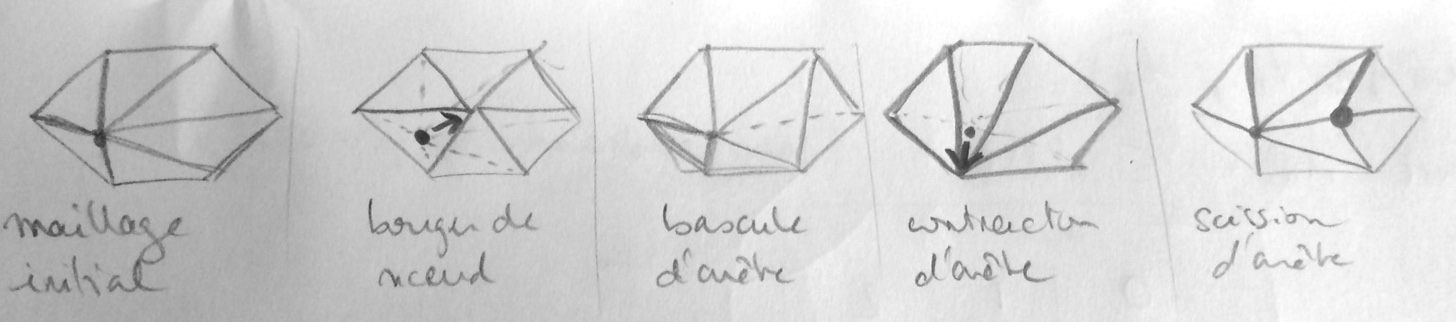
\includegraphics[width=\textwidth]{operations_locales_optimisation_maillage}
	\begin{tikzpicture}[
		x=\imagewidth,
		y=\imageheight,
		mesh/.style={draw=black, semithick},
		label/.style={anchor=south west, inner sep=0},
		optim/.style={mycolor_2, line width=2.0pt},
		arrow/.style={optim , -stealth}, 
		move/.style={arrow, shorten <=2pt, shorten >=3pt},
		swap/.style={arrow, shorten <=1pt, shorten >=1pt},
		%collapse/.style={arrow, shorten <=2pt, shorten >=3pt},
		collapse/.style={optim, dashed},
		before/.style={draw=black!30!white, dashed, thin},
		vertex/.style={fill=black, draw=none, circle, scale=0.3, inner sep=0},
	]
		\begin{scope}[shift={(0.0, -0)}]
	\draw[mesh] 
		(0.08373422920703888, 0.9040214419364929) -- (-0.8304623365402222, 0.49192529916763306)
		(-0.5802370309829712, 0.24899999797344208) -- (0.8759713172912598, -0.40999728441238403)
		(-0.5802370309829712, 0.24899999797344208) -- (0.08373422920703888, 0.9040214419364929)
		(-0.5802370309829712, 0.24899999797344208) -- (0.8661928772926331, 0.48200759291648865)
		(0.8759713172912598, -0.40999728441238403) -- (0.8661928772926331, 0.48200759291648865)
		(-0.5802370309829712, 0.24899999797344208) -- (-0.8304623365402222, 0.49192529916763306)
		(0.0585169717669487, -0.770743727684021) -- (0.8759713172912598, -0.40999728441238403)
		(0.08373422920703888, 0.9040214419364929) -- (0.8661928772926331, 0.48200759291648865)
		(-0.5802370309829712, 0.24899999797344208) -- (-0.7628560066223145, -0.4127168357372284)
		(-0.8304623365402222, 0.49192529916763306) -- (-0.7628560066223145, -0.4127168357372284)
		(-0.5802370309829712, 0.24899999797344208) -- (0.0585169717669487, -0.770743727684021)
		(-0.7628560066223145, -0.4127168357372284) -- (0.0585169717669487, -0.770743727684021)
		;
	\node[label] at (-0.866025403784, -0.83) {(a)};
\end{scope}
\begin{scope}[shift={(1.19802540378, -1.82004086811)}]
	\draw[before] 
		(0.08373422920703888, 0.9040214419364929) -- (-0.8304623365402222, 0.49192529916763306)
		(-0.5802370309829712, 0.24899999797344208) -- (0.8759713172912598, -0.40999728441238403)
		(-0.5802370309829712, 0.24899999797344208) -- (0.08373422920703888, 0.9040214419364929)
		(-0.5802370309829712, 0.24899999797344208) -- (0.8661928772926331, 0.48200759291648865)
		(0.8759713172912598, -0.40999728441238403) -- (0.8661928772926331, 0.48200759291648865)
		(-0.5802370309829712, 0.24899999797344208) -- (-0.8304623365402222, 0.49192529916763306)
		(0.0585169717669487, -0.770743727684021) -- (0.8759713172912598, -0.40999728441238403)
		(0.08373422920703888, 0.9040214419364929) -- (0.8661928772926331, 0.48200759291648865)
		(-0.5802370309829712, 0.24899999797344208) -- (-0.7628560066223145, -0.4127168357372284)
		(-0.8304623365402222, 0.49192529916763306) -- (-0.7628560066223145, -0.4127168357372284)
		(-0.5802370309829712, 0.24899999797344208) -- (0.0585169717669487, -0.770743727684021)
		(-0.7628560066223145, -0.4127168357372284) -- (0.0585169717669487, -0.770743727684021)
		;
	\draw[mesh] 
		(0.08373422920703888, 0.9040214419364929) -- (-0.8304623365402222, 0.49192529916763306)
		(0.0485161654651165, 0.0474160760641098) -- (0.8759713172912598, -0.40999728441238403)
		(0.0485161654651165, 0.0474160760641098) -- (0.08373422920703888, 0.9040214419364929)
		(0.0485161654651165, 0.0474160760641098) -- (0.8661928772926331, 0.48200759291648865)
		(0.8759713172912598, -0.40999728441238403) -- (0.8661928772926331, 0.48200759291648865)
		(0.0485161654651165, 0.0474160760641098) -- (-0.8304623365402222, 0.49192529916763306)
		(0.0585169717669487, -0.770743727684021) -- (0.8759713172912598, -0.40999728441238403)
		(0.08373422920703888, 0.9040214419364929) -- (0.8661928772926331, 0.48200759291648865)
		(0.0485161654651165, 0.0474160760641098) -- (-0.7628560066223145, -0.4127168357372284)
		(-0.8304623365402222, 0.49192529916763306) -- (-0.7628560066223145, -0.4127168357372284)
		(0.0485161654651165, 0.0474160760641098) -- (0.0585169717669487, -0.770743727684021)
		(-0.7628560066223145, -0.4127168357372284) -- (0.0585169717669487, -0.770743727684021)
		;
	\fill[black] (0.0485161654651165,0.0474160760641098) circle (\vertexradius);
	\draw[move] (-0.5802370309829712,0.24899999797344208) -- (0.0485161654651165,0.0474160760641098);
	\node[label] at (-0.866025403784, -0.83) {(b)};
\end{scope}
\begin{scope}[shift={(2.39605080757, -0)}]
	\draw[before] 
		(0.08373422920703888, 0.9040214419364929) -- (-0.8304623365402222, 0.49192529916763306)
		(-0.5802370309829712, 0.24899999797344208) -- (0.8759713172912598, -0.40999728441238403)
		(-0.5802370309829712, 0.24899999797344208) -- (0.08373422920703888, 0.9040214419364929)
		(-0.5802370309829712, 0.24899999797344208) -- (0.8661928772926331, 0.48200759291648865)
		(0.8759713172912598, -0.40999728441238403) -- (0.8661928772926331, 0.48200759291648865)
		(-0.5802370309829712, 0.24899999797344208) -- (-0.8304623365402222, 0.49192529916763306)
		(0.0585169717669487, -0.770743727684021) -- (0.8759713172912598, -0.40999728441238403)
		(0.08373422920703888, 0.9040214419364929) -- (0.8661928772926331, 0.48200759291648865)
		(-0.5802370309829712, 0.24899999797344208) -- (-0.7628560066223145, -0.4127168357372284)
		(-0.8304623365402222, 0.49192529916763306) -- (-0.7628560066223145, -0.4127168357372284)
		(-0.5802370309829712, 0.24899999797344208) -- (0.0585169717669487, -0.770743727684021)
		(-0.7628560066223145, -0.4127168357372284) -- (0.0585169717669487, -0.770743727684021)
		;
	\draw[mesh] 
		(0.08373422920703888, 0.9040214419364929) -- (-0.8304623365402222, 0.49192529916763306)
		(-0.5802370309829712, 0.24899999797344208) -- (0.8759713172912598, -0.40999728441238403)
		(-0.5802370309829712, 0.24899999797344208) -- (0.08373422920703888, 0.9040214419364929)
		(-0.5802370309829712, 0.24899999797344208) -- (0.8661928772926331, 0.48200759291648865)
		(0.8759713172912598, -0.40999728441238403) -- (0.8661928772926331, 0.48200759291648865)
		(-0.5802370309829712, 0.24899999797344208) -- (-0.8304623365402222, 0.49192529916763306)
		(0.0585169717669487, -0.770743727684021) -- (0.8759713172912598, -0.40999728441238403)
		(0.08373422920703888, 0.9040214419364929) -- (0.8661928772926331, 0.48200759291648865)
		(-0.5802370309829712, 0.24899999797344208) -- (-0.7628560066223145, -0.4127168357372284)
		(-0.8304623365402222, 0.49192529916763306) -- (-0.7628560066223145, -0.4127168357372284)
		(-0.7628560066223145, -0.4127168357372284) -- (0.0585169717669487, -0.770743727684021)
		(0.8759713172912598, -0.40999728441238403) -- (-0.7628560066223145, -0.4127168357372284)
		;
	\draw[swap] (-0.26086002588272095,-0.26087185740470886) to [bend left=\swapbend] (0.056557655334472656,-0.411357045173645);
	\node[label] at (-0.866025403784, -0.83) {(c)};
\end{scope}
\begin{scope}[shift={(3.59407621135, -1.82004086811)}]
	\draw[before] 
		(0.08373422920703888, 0.9040214419364929) -- (-0.8304623365402222, 0.49192529916763306)
		(-0.5802370309829712, 0.24899999797344208) -- (0.8759713172912598, -0.40999728441238403)
		(-0.5802370309829712, 0.24899999797344208) -- (0.08373422920703888, 0.9040214419364929)
		(-0.5802370309829712, 0.24899999797344208) -- (0.8661928772926331, 0.48200759291648865)
		(0.8759713172912598, -0.40999728441238403) -- (0.8661928772926331, 0.48200759291648865)
		(-0.5802370309829712, 0.24899999797344208) -- (-0.8304623365402222, 0.49192529916763306)
		(0.0585169717669487, -0.770743727684021) -- (0.8759713172912598, -0.40999728441238403)
		(0.08373422920703888, 0.9040214419364929) -- (0.8661928772926331, 0.48200759291648865)
		(-0.5802370309829712, 0.24899999797344208) -- (-0.7628560066223145, -0.4127168357372284)
		(-0.8304623365402222, 0.49192529916763306) -- (-0.7628560066223145, -0.4127168357372284)
		(-0.5802370309829712, 0.24899999797344208) -- (0.0585169717669487, -0.770743727684021)
		(-0.7628560066223145, -0.4127168357372284) -- (0.0585169717669487, -0.770743727684021)
		;
	\draw[mesh] 
		(-0.8304623365402222, 0.49192529916763306) -- (0.8759713172912598, -0.40999728441238403)
		(-0.8304623365402222, 0.49192529916763306) -- (0.08373422920703888, 0.9040214419364929)
		(-0.8304623365402222, 0.49192529916763306) -- (0.8661928772926331, 0.48200759291648865)
		(0.8759713172912598, -0.40999728441238403) -- (0.8661928772926331, 0.48200759291648865)
		(0.0585169717669487, -0.770743727684021) -- (0.8759713172912598, -0.40999728441238403)
		(0.08373422920703888, 0.9040214419364929) -- (0.8661928772926331, 0.48200759291648865)
		(-0.8304623365402222, 0.49192529916763306) -- (-0.7628560066223145, -0.4127168357372284)
		(-0.8304623365402222, 0.49192529916763306) -- (0.0585169717669487, -0.770743727684021)
		(-0.7628560066223145, -0.4127168357372284) -- (0.0585169717669487, -0.770743727684021)
		;
	\draw[collapse] (-0.5802370309829712,0.24899999797344208) -- (-0.8304623365402222,0.49192529916763306);
	\node[label] at (-0.866025403784, -0.83) {(d)};
\end{scope}
\begin{scope}[shift={(4.79210161514, -0)}]
	\draw[mesh] 
		(0.08373422920703888, 0.9040214419364929) -- (-0.8304623365402222, 0.49192529916763306)
		(0.1478671431541443, -0.08049865067005157) -- (0.8759713172912598, -0.40999728441238403)
		(-0.5802370309829712, 0.24899999797344208) -- (0.08373422920703888, 0.9040214419364929)
		(-0.5802370309829712, 0.24899999797344208) -- (0.8661928772926331, 0.48200759291648865)
		(0.8759713172912598, -0.40999728441238403) -- (0.8661928772926331, 0.48200759291648865)
		(-0.5802370309829712, 0.24899999797344208) -- (-0.8304623365402222, 0.49192529916763306)
		(0.0585169717669487, -0.770743727684021) -- (0.8759713172912598, -0.40999728441238403)
		(0.08373422920703888, 0.9040214419364929) -- (0.8661928772926331, 0.48200759291648865)
		(-0.5802370309829712, 0.24899999797344208) -- (-0.7628560066223145, -0.4127168357372284)
		(-0.8304623365402222, 0.49192529916763306) -- (-0.7628560066223145, -0.4127168357372284)
		(-0.5802370309829712, 0.24899999797344208) -- (0.0585169717669487, -0.770743727684021)
		(-0.7628560066223145, -0.4127168357372284) -- (0.0585169717669487, -0.770743727684021)
		(0.1478671431541443, -0.08049865067005157) -- (-0.5802370309829712, 0.24899999797344208)
		(0.1478671431541443, -0.08049865067005157) -- (0.8661928772926331, 0.48200759291648865)
		(0.0585169717669487, -0.770743727684021) -- (0.1478671431541443, -0.08049865067005157)
		;
	\fill[black] (0.1478671431541443,-0.08049865067005157) circle (\vertexradius);
	\node[label] at (-0.866025403784, -0.83) {(e)};
\end{scope}

	\end{tikzpicture}
	\caption{Opérations élémentaires d'optimisation de maillage surfacique. (a) Maillage initial. (b) Bouger de n\oe ud. (c) Bascule d'arête. (d) Contraction d'arête. (e) Scission d'arête (insertion de n\oe ud).}
	\label{fig:operations_locales_optimisation_maillage}
\end{figure}